\subsection{Distribution fitting by maximum likelihood : {\tt fitdistr\index{fitdistr}}}
{\tt fitdistr} takes two arguments, a list $L$ of presumably independent and identically distributed samples and a distribution type, which may be normal, exponential, Poisson, geometric, gamma, beta, Cauchy or Weibull. The type is specified as {\tt normal} ({\tt normald}), {\tt exp} ({\tt exponential} or {\tt exponentiald}), {\tt poisson}, {\tt geometric}, {\tt gammad}, {\tt betad}, {\tt cauchy} ({\tt cauchyd}) or {\tt weibull} ({\tt weibulld}), respectively. The command returns the distribution of the specified type with parameters that fit the given samples most closely according to the method of maximum likelihood.

For example, input :
\begin{center}
  \tt S:=randvector(1000,weibulld,1/2,1):; fitdistr(S,weibull)
\end{center}
Output :
\begin{center}
  \tt weibulld(0.498920254339,0.971148738409)
\end{center}
Input :
\begin{center}
  \tt X:=randvar(normal,stddev=9.5):; Y:=randvar(normal,stddev=1.5):; S:=sample(eval(X/Y,0),1000):; Z:=fitdistr(S,cauchy)
\end{center}
Output :
\begin{center}
  \tt cauchyd(-0.13160176167,6.2569300393)
\end{center}
Input :
\begin{center}
  \tt histogram(select(x->(x>-100 and x<100),S)); plot(Z(x),x=-100..100,display=red+line\_width\_2)
\end{center}
Output :
\begin{center}
  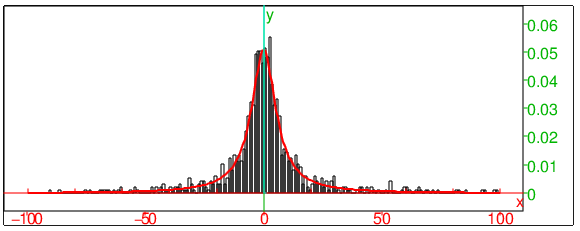
\includegraphics[width=0.75\textwidth]{fitdistr.png}
\end{center}
Input :
\begin{center}
  \tt kolmogorovt(S,Z)
\end{center}
Output :
\begin{center}
  \tt ["D=",0.0125864995943,"K=", 0.398020064869, "1-kolmogorovd(K)=",0.997387219452]
\end{center}
The Kolmogorov-Smirnov test indicates that the samples from $S$ are drawn from $Z$ with high probability.

Fitting a lognormal distribution to samples $x_1,x_2,\dots,x_n$ can be done by fitting a normal distribution to the sample logarithms $\log x_1,\log x_2,\dots,\log x_n$ because log-likelihood functions are the same. For example, generate some samples according to the lognormal rule with parameters $\mu=5$ and $\sigma^2=2$ :
\begin{center}
  \tt X:=randvar(normal,mean=5,variance=2):; S:=sample(exp(X),1000):;
\end{center}
Now fit normal distribution to $\log S$ :
\begin{center}
  \tt Y:=fitdistr(log(S),normal)
\end{center}
Output :
\begin{center}
  \tt normald(5.04754808715,1.42751619912)
\end{center}
The mean of $Y$ is about $5.05$ and the variance is about $2.04$. Now the variable $Z=\exp(Y)$ has the sought lognormal distribution.
